\subsection*{Exercise 1}

Build the connection matrix $B\in \mathbb{R}^{5 \times 5}$ relative to the web
made of the 5 pages, as depicted in Fig.~\ref{fig:web}.
%
\begin{figure}
\centering
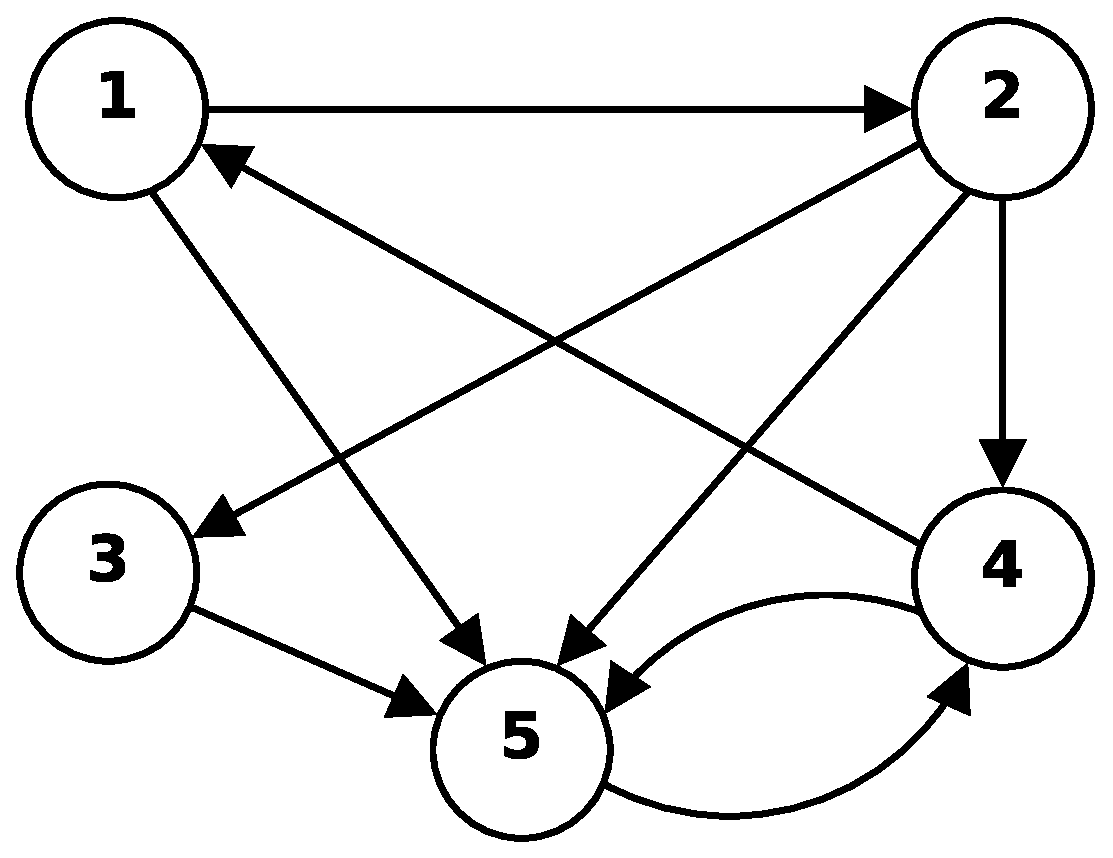
\includegraphics[width=0.35\textwidth]{fig/web}
\caption{Scheme for a 5 pages web. Every circle is a page, every arrow is a
link.}
\label{fig:web}
\end{figure}
%
Using the \texttt{Eigen} library, write down a class that computes the maximum
eigenvalue (that is 1) and the corresponding eigenvector, that is the
\emph{pagerank}. Implement also \cpp{operator<<} to see the data inside the
class on the screen.
